%%%%%%%%%%%%%%%%%%%%%%%%%%%%%%%%%%%%%%%%%%%%%%%%%%%%%%%%%%%%%%%%%%%%
%% I, the copyright holder of this work, release this work into the
%% public domain. This applies worldwide. In some countries this may
%% not be legally possible; if so: I grant anyone the right to use
%% this work for any purpose, without any conditions, unless such
%% conditions are required by law.
%%%%%%%%%%%%%%%%%%%%%%%%%%%%%%%%%%%%%%%%%%%%%%%%%%%%%%%%%%%%%%%%%%%%

\documentclass{beamer}
\usepackage[utf8]{inputenc}
\usepackage{tikz}
\usetikzlibrary{shapes.geometric, arrows}
\usetheme[faculty=fi,logoPath=logo/,logo=logo/LOGO.pdf]{fibeamer}
\usepackage[
main=english, %% By using `czech` or `slovak` as the main locale
%% instead of `english`, you can typeset the
%% presentation in either Czech or Slovak,
%% respectively.
italian %% The additional keys allow foreign texts to be
]{babel}        %% typeset as follows:
%%
%%   \begin{otherlanguage}{czech}   ... \end{otherlanguage}
%%   \begin{otherlanguage}{slovak}  ... \end{otherlanguage}
%%
%% These macros specify information about the presentation
\title{An extension of FJ to interfaces and intersection types} %% that will be typeset on the
\subtitle{Syntax, typing, subtyping and evaluation rules} %% title page.
\author{Cosimo Cinquilli \& Gabriele Giannini}
%% These additional packages are used within the document:
\usepackage{ragged2e}  % `\justifying` text
\usepackage{booktabs}  % Tables
\usepackage{tabularx}
\usepackage{tikz}      % Diagrams
\usetikzlibrary{calc, shapes, backgrounds}
\usepackage{amsmath, amssymb}
\usepackage{url}       % `\url`s
\usepackage{listings}  % Code listings

\usepackage{mathtools}
\usepackage{xargs}
\usepackage{esvect}
\usepackage{listings}
\usepackage{color}
\usepackage{bm}

\definecolor{dkgreen}{rgb}{0,0.6,0}
\definecolor{gray}{rgb}{0.5,0.5,0.5}
\definecolor{mauve}{rgb}{0.58,0,0.82}

\lstset{frame=tb,
	language=Java,
	aboveskip=3mm,
	belowskip=3mm,
	showstringspaces=false,
	columns=flexible,
	basicstyle={\small\ttfamily},
	numbers=none,
	numberstyle=\tiny\color{gray},
	keywordstyle=\color{blue},
	commentstyle=\color{dkgreen},
	stringstyle=\color{mauve},
	breaklines=true,
	breakatwhitespace=true,
	tabsize=3
}

\newcommand{\syntaxtag}[1]{{\textit{#1}}}
\newcommand{\syntaxkeyword}[1]{\texttt{#1}}
\newcommand{\aargs}[1]{\vv #1}

% un bello spazio verticale per evitare che le cose nelle frazioni siano appiccicate fra loro
\newcommand{\hs}{\vphantom{\tilde{\aargs{I}}}}

% la class declaration
\newcommand{\iclass}[3]{\syntaxkeyword{class } #1 \syntaxkeyword{ extends } #2 \syntaxkeyword{ implements } \aargs #3 \; \{ \aargs T \, \aargs f ; \; K \; \aargs M \} \hs}
% l'interface declaration
\newcommandx{\einterface}[2][2=I]{\syntaxkeyword{interface } #1 \syntaxkeyword{ extends } \aargs #2 \;\{ \aargs S\} \hs }
% \newcommand{\mathlarge}[1]{\mbox{\LARGE $#1$}}
\newcommand{\mathlarge}[1]{\displaystyle {#1}}
\newcommand{\onto}[1]{\atop \mathlarge{#1}}
\newcommand{\sig}{\Sigma ig}


\frenchspacing
\begin{document}
	\frame{\maketitle}
	
	\AtBeginSection[]{% Print an outline at the beginning of sections
		\begin{frame}<beamer>
		\frametitle{Outline for Section \thesection}
		\footnotesize
		\tableofcontents[currentsection]
\end{frame}}

%  \AtBeginSection[]{% Print an outline at the beginning of sections
%    \begin{frame}<beamer>
%      \frametitle{Outline for Section \thesection}
%      \tableofcontents[currentsection]
%    \end{frame}}


    \section{Extending FJ to interfaces: FIJ}

    \begin{frame}
      \frametitle{Extending FJ to interfaces: FIJ}
      \framesubtitle{The final objective}
      We wanto to introduce interfaces in FJ in order to be able to have a more
      sophisticated structure of the types relation (no more a simple tree).

      We want obviously to maintain the core functionality that we have already, just adding interfaces
      on top of that. Moreover, we want to rest sure that every FIJ program is indeed a valid Java
      program, as it was the case for FJ.
    \end{frame}

    \begin{frame}
      \frametitle{Simbols and their meanings}
      \framesubtitle{Let's get the notation clear}
        \begin{columns}[onlytextwidth]
          \column{.5\textwidth}
              $I, J$ = interface names\\[5pt]
              $C, D$ = class names\\[5pt]
              $T, U, V$ = types literals\\[5pt]
              $\aargs S, \Sigma, S, Z$ = sets of signatures\\[5pt]
              $\aargs M$ = methods declarations\\[5pt]
              % $K$ = constructor\\
              $\aargs f, \aargs g$ = fields\\[5pt]
              $\aargs x$ = formal parameters\\
            \column{.5\textwidth}
              $\aargs a$ = \parbox{.6\textwidth}{generic list or set of elements as $a$}
              % \begin{flalign*} % allineato alla prima riga
              %   \aargs{I} = \; I_1,&\dots,I_n \;\; or\\
              %   I_1\&&\dots\&I_n
              % \end{flalign*}
              \begin{flalign*} % centrato verticalmente
                &\aargs{I} = {\hspace{15pt} I_1,\dots,I_n \;\; or\atop{
                I_1\&\dots\&I_n}}&
                \parbox{40pt}{\scriptsize{(specific for\\ interfaces)}}
              \end{flalign*}\\
              $T \in \aargs T \Leftrightarrow \aargs T = T_1,\dots,T,\dots,T_n$\\[5pt]
              $T<:\aargs U \Leftrightarrow T<:U \;\;\; \forall U \in \aargs U$\\[5pt]
              $\aargs T = \aargs U \Leftrightarrow T_i = U_i \;\,for\ 1\leq i\leq n$
        \end{columns}
    \end{frame}

    \subsection{Extending the syntax}
    \begin{frame}{The new syntax (1/3)}
      \framesubtitle{Classes, interfaces, method signatures}
      \vspace{-10pt}
      \begin{flalign*}
          IN &::= \hspace{175pt}\syntaxtag{interface declaration}&\\
          &\qquad \einterface{I} &\\[10pt]
          S &::= \hspace{136pt}\syntaxtag{method signature declaration}&\\
          &\qquad T \; m(\aargs T \ \aargs x);&\\[10pt]
          CL &::= \hspace{193pt}\syntaxtag{class declaration}&\\
          &\qquad \iclass{C}{C}{I}&\\
        \end{flalign*}
      \end{frame}

      \begin{frame}{The new syntax (2/3)}
        \framesubtitle{Constructor, methods, types}
        \begin{flalign*}
          K &::= \hspace{165pt}\syntaxtag{constructor declaration}&\\
          &\qquad C(\aargs T \ \aargs f\,) \ \{\,\syntaxkeyword{super}(\aargs f\,); \; \syntaxkeyword{this}.\aargs f = \aargs f;\,\}&\\[10pt]
          M &::= \hspace{138pt}\syntaxtag{complete method declaration}&\\
          &\qquad T \; m(\aargs T \ \aargs x) \ \{\,\syntaxkeyword{return } t;\,\}&\\[10pt]
          T &::= \hspace{220pt}\syntaxtag{type literal}&\\
          &\qquad C \; | \; I &\\
        \end{flalign*}
      \end{frame}

      \begin{frame}{The new syntax (3/3)}
        \framesubtitle{Terms, values}
        \vspace{-10pt}
        \begin{flalign*}
          t &::= &\syntaxtag{terms:}\\
          &\qquad x &\syntaxtag{variables}\\
          &\qquad t.f &\syntaxtag{field access}\\
          &\qquad t.m(\aargs t) &\syntaxtag{method invocation}\\
          &\qquad \syntaxkeyword{new } C(\aargs t) &\syntaxtag{object creation}\\
          &\qquad (T) \ t &\syntaxtag{cast}\\[10pt]
          v &::= &\syntaxtag{values:}\\
          &\qquad \syntaxkeyword{new } C(\aargs v) &\syntaxtag{object creation}
      \end{flalign*}
    \end{frame}

    \subsection{Extending the subtype relation}
    \begin{frame}
      \frametitle{Extending the definition of the subtype relation}

      \begin{definition}
        \vspace{-25pt}
        \begin{flalign*}
          &T<:T &\\[5pt]
          &\dfrac{T<:U \qquad U<:V}{T<:V} &\\
          &\dfrac{\mathlarge{CT(C) = \iclass{C}{D}{I}}}{C<:D \quad C<:\aargs I} &\\
          &\dfrac{CT(I) = \einterface{I}[J]}{I<: \aargs{J}} &
          % &\dfrac{CT(C) = \iclass{C}{D}{I}}{C<:\aargs{I}} &
      \end{flalign*}
      \end{definition}
    \end{frame}

    \subsection{Auxiliary functions}

    \begin{frame}{Preparing for extension}
     \boldmath
      % \framesubtitle{Adding some auxiliary functions}
      We add the $IObject$ type: as $Object$ is the supertype of every class,
      so $IObject$ is an empty interface outside the Class Table that is the
      supertype of every interface.

      We then define a new function $\sig$ on classes and groups of interfaces, we define also a new
      predicate $is\sig ok$ on sets of signatures and we redefine $mtype$ also for interfaces.
    \end{frame}

    \subsubsection{$is\sig ok$ predicate}
    \begin{frame}
      \frametitle{$is\sig ok$ predicate}
      \framesubtitle{Defined on a set of signatures}
      This helper predicate is $true$ if and only if the set of signatures is actually an interface,
      that is, for any method name in it, it contains \alert{only one} signature for that name.
      \begin{definition}
        \vspace{-20pt}
        \begin{flalign*}
          &\dfrac{
            T\ m(\aargs T\ \aargs x);\in\Sigma \land U\ m(\aargs U\ \aargs{y});\in\Sigma
            \;\;\alert{\text{ implies }}\;\; T=U \land \aargs{T}=\aargs{U}
          }{is\sig ok(\Sigma)}
        \end{flalign*}
      \end{definition}
    \end{frame}

    \subsubsection{$\sig$ function}

    \begin{frame}{$\sig$ function}
      \framesubtitle{For interfaces and groups of interfaces}
      \begin{definition}
        \vspace{-20pt}
        \begin{flalign*}
          &\sig(IObject)=\emptyset &\\[10pt]
          % &\dfrac{\mathlarge{
          %     CT(I)=\einterface{I}[J] \atop
          %     \sig(\aargs{J}) = \aargs{S}
          % }}{\sig(I) = \aargs{S} \cup \aargs{N} \hs} &\\[10pt]
          % &\dfrac{\mathlarge{
          %     I \in \aargs{I} \quad \sig(I) = \aargs S \quad \sig(\aargs I \setminus \{I\}) = \aargs R
          % }}{\sig(\aargs I) = \aargs S \cup \aargs R}
          &\dfrac{
            \mathlarge{
              CT(I) = \einterface{I}[J] \atop
              % \Sigma = \sig(J_1)\cup\dots\cup\sig(J_n)\cup\aargs N
              \Sigma = \sig(J_1,\dots, J_n)
            }
          }{\sig(I) = \Sigma \cup\aargs S}&\\[10pt]
          &\dfrac{
            \mathlarge{
              \Sigma = \sig(I_1)\cup\dots\cup\sig(I_n)
              % \qquad is\sig ok(\Sigma)
            }
          }{\sig(I_1, \dots, I_n) = \Sigma}&
      \end{flalign*}
      \end{definition}
    \end{frame}

    \begin{frame}{$\sig$ function}
      \framesubtitle{For classes}
      \begin{definition}
        \vspace{-20pt}
        \begin{flalign*}
          &\sig(Object) = \emptyset &\\[5pt]
          &\dfrac{\mathlarge{
                CT(C) = \iclass{C}{D}{I}
                \onto{ \Sigma = \bigl\{ U \;\; m(\aargs U \ \aargs x); \; \big| \; U \;\; m(\aargs U \ \aargs x) \{\syntaxkeyword{return } t;\} \in \aargs{M} \bigr\}
                \onto{\sig(D) = S}
                % \qquad \sig(\aargs I) = Z
              }
          }}{\sig(C)=\Sigma \cup S \hs}&
      \end{flalign*}
      \end{definition}
      % \scriptsize{
      % \begin{alertblock}{Note}
      %   We include the signatures of the implemented interfaces. This will be useful later when
      %   dealing with the typing of classes.
      % \end{alertblock}}
    \end{frame}

    \subsubsection{mtype function}
    \begin{frame}
      \frametitle{mtype function}
      % \framesubtitle{For interfaces}
      \begin{definition}
        \vspace{-20pt}
        \begin{flalign*}
          % &\dfrac{
          %   CT(I) = \einterface{I} \quad T \ m(\aargs T \ \aargs x); \in \aargs S
          % }
          % {mtype(m,I) = \aargs T \rightarrow T \hs} &\\[10pt]
          % &\dfrac{
          %   \mathlarge{ % \mathlarge per evitare che le cose scritte sotto \atop vengano piccoline
          %     CT(I) = \einterface{I}
          %     \atop m \text{ is not in declared in } I \qquad T\ m(\aargs T\ \aargs x); \in \sig(\aargs I)
          %   }
          % }
          % {mtype(m,I) = \aargs T \rightarrow T}
          % &&\syntaxtag{(for interfaces)}\\[-25pt]
          % &\dfrac{
          %     T\ m(\aargs T\ \aargs x);\, \in\, \sig(I)
          % }
          % {mtype(m,I) = \aargs T \rightarrow T}&\\[10pt]
          % &&\syntaxtag{(for classes)}\\[-22pt]
          % &\dfrac{
          %   T\ m(\aargs T\ \aargs x);\,\in\,\sig(C)
          % }{mtype(m, C)=\aargs T \rightarrow T}
          &\dfrac{
            U\ m(\aargs U\ \aargs x);\,\in\,\sig(T)
          }{mtype(m, T)=\aargs U \rightarrow U}
          % \\[5pt]
          % &\dfrac{
          %   % \mathlarge
          %   {
          %     CT(C)=\iclass{C}{D}{I} \atop
          %     T\ m(\aargs T\ \aargs x);\,\{\syntaxkeyword{return }t;\} \in\, \aargs M
          %   }
          % }{mtype(m,C) = \aargs T \rightarrow T}&
        \end{flalign*}
      \end{definition}
      \small{
        \begin{alertblock}{Note}
        \boldmath
          The $\sig$ function greatly simplify the definition of $mtype$.\\
          % Please, also note that with this definition if a class $C$ doesn't implement a method body for $m$,
          % a method declared in an implemented interface, $mtype(m,C)$ will still be defined, returning
          % the expected type for the method. This is not a problem, we will see that we can use $mbody$ to correctly
          % check this.
          %
          Also note that, as was the case in FJ, $mtype(m,C)$ is not defined if the method $m$ is not implemented
          in $C$ or any of its superclasses.
        \end{alertblock}
      }
    \end{frame}

    % \subsubsection{$mbody$ function}

    \begin{frame}{$mbody$ function}
      \framesubtitle{Just a recall of the definition}
      \begin{definition}
        \vspace{-20pt}
        \begin{flalign*}
          &\dfrac{
            \mathlarge{
              CT(C) = \iclass{C}{D}{I} \atop
              T\ m(\aargs T\ \aargs x)\; \{\syntaxkeyword{return }t;\}\,\in\aargs M
            }
          }{mbody(m,C) = (\aargs x, t)}&\\[10pt]
          &\dfrac{
            \mathlarge{
              CT(C)=\iclass{C}{D}{I}
              \atop m\text{ is not defined in }\aargs M
            }
          }{mbody(m,C) = mbody(m,D)}&
      \end{flalign*}
      \end{definition}
    \end{frame}

    % \begin{frame}
    %   \frametitle{mtype function}
    %   \framesubtitle{For classes}
    %   \begin{definition}
    %     \vspace{-20pt}
    %     \begin{flalign*}
    %       &\dfrac{
    %         \mathlarge{ % \mathlarge per evitare che le cose scritte sotto \atop vengano piccoline
    %           CT(C) = \iclass{C}{D}{I}
    %           \atop C \ m(\aargs C \ \aargs x); \in \aargs N
    %         }
    %       }
    %       {
    %         mtype(m,C) = \aargs C \rightarrow C \hs} &\\[10pt] %a capo di 10 punti per fare spazio
    %       &\dfrac{
    %         \mathlarge{
    %           CT(C) = \iclass{C}{D}{I}
    %           \atop m \text{ is not in declared in } I \hs
    %         }
    %       }
    %       {mtype(m,C) = mtype(m,D)}
    %   \end{flalign*}
    %   \end{definition}
    % \end{frame}

    % \begin{frame}
    %   \frametitle{names function}
    %   % \framesubtitle{}
    %   Really small function, but it let us define the next predicate, $compatible$, in a more
    %   compact and readable way.
    %   \begin{definition}
    %     \vspace{-20pt}
    %     \begin{flalign*}
    %       &\dfrac{
    %         \mathlarge{ % \mathlarge per evitare che le cose scritte sotto \atop vengano piccoline
    %           P = \{m\; \big| \; T\; m(\aargs T \ \aargs x); \in signatures(\aargs I)\}
    %         }
    %       }
    %       {names(\aargs I) = P}
    %   \end{flalign*}
    %   \end{definition}
    % \end{frame}

    % \subsubsection{compatible predicate}
    % \begin{frame}
    %   \frametitle{compatible predicate}
    %   \framesubtitle{Defined on groups of interfaces}
    %   \vspace{-5pt}
    %   \begin{definition}
    %     \vspace{-30pt}
    %     \begin{flalign*}
    %       % &\dfrac{
    %       %   \mathlarge{
    %       %     I \in \aargs I \qquad \aargs J = \aargs I \setminus \{I\} \qquad compatible(\aargs{J})
    %       %     \onto{
    %       %       (T\; m(\aargs{T}\ \aargs x); \in signatures(\aargs J) \text{ implies } mtype(m, I) \text{ not defined}
    %       %       \onto{
    %       %         \text{or } T\; m(\aargs T\ \aargs x); \in signatures(\aargs J) \land mtype(m, I) = \aargs T \rightarrow T)
    %       %       }
    %       %     }
    %       %   }
    %       % }
    %       % &\dfrac{
    %       %   \mathlarge{
    %       %     I \in \aargs I \qquad \aargs J = \aargs I \setminus \{I\} \qquad compatible(\aargs{J})
    %       %     \onto{ P = \{m\; \big| \; T\; m(\aargs T \ \aargs x); \in signatures(\aargs I)\} \qquad m\in P
    %       %       \onto{
    %       %         (mtype(m,\aargs J)=\aargs U \rightarrow U \text{ implies } mtype(m, I) \text{ not defined}
    %       %         \onto{
    %       %           \text{or } mtype(m,\aargs J)=\aargs U \rightarrow U \land mtype(m, I) = \aargs U \rightarrow U)
    %       %         }
    %       %       }
    %       %     }
    %       %   }
    %       % }
    %       &\dfrac{}{compatible(I)}\\[10pt]
    %       &\dfrac{
    %         \mathlarge{
    %           I \in \aargs I \qquad \aargs J = \aargs I \setminus \{I\} \qquad compatible(\aargs{J}) \qquad m\in names(\aargs I)
    %             \onto{
    %               mtype(m,\aargs J)=\aargs U \rightarrow U \;\; \alert{\text{implies}}\;\; mtype(m, I) \;\;\alert{\text{not defined}}
    %             }
    %         }
    %       }
    %       {compatible(\aargs I) \hs}\\[10pt]
    %       &\dfrac{
    %         \mathlarge{
    %           I \in \aargs I \qquad \aargs J = \aargs I \setminus \{I\} \qquad compatible(\aargs{J}) \qquad m\in names(\aargs I)
    %             \onto{
    %                 mtype(m,\aargs J)=\aargs U \rightarrow U \qquad mtype(m, I) = \aargs U \rightarrow U \hs
    %             }
    %         }
    %       }
    %       {compatible(\aargs I) \hs}
    %     \end{flalign*}
    %   \end{definition}
    % \end{frame}

    \subsection{Extending the typing rules}

    \begin{frame}
      \frametitle{The new typing rules}
      \vspace{-30pt}
      \begin{flalign*}
        &&\syntaxtag{(T-VAR)} \\[-20pt]
        &\dfrac{ x:T \in \Gamma }{ \Gamma \vdash x:T } &\\[10pt]
        &&\syntaxtag{(T-FIELD)} \\[-20pt]
        &\dfrac{ \Gamma \vdash t_0 : C_0 \qquad fields(C_0) = \aargs T \; \aargs f}
        {\Gamma \vdash t_0 . f_i : T_i }&\\[10pt]
        &&\syntaxtag{(T-UCAST)} \\[-20pt]
        &\dfrac{ \Gamma \vdash t_0 : U \qquad U <: T}
        { \Gamma \vdash (T)\, t_0 : T} &\\[10pt]
        &&\syntaxtag{(T-DCAST)} \\[-20pt]
        &\dfrac{ \Gamma \vdash t_0:U \qquad T <: U \qquad T \neq U}
        { \Gamma \vdash (T)\, t_0:T}
    \end{flalign*}
    \end{frame}

    \begin{frame}
      \frametitle{The new typing rules}
      \vspace{-30pt}
      \begin{flalign*}
        &&\syntaxtag{(T-INVK)} \\[-20pt]
        &\dfrac{
          \mathlarge{
            \Gamma \vdash t_0:C_0 \qquad mtype(m, C_0) = \aargs U \rightarrow T
            \atop
            \Gamma \vdash \aargs t:\aargs T \qquad \aargs T <: \aargs U \hs
          }
        }{ \Gamma \vdash t_0.m(\aargs t): T \hs} &\\[10pt]
        &&\syntaxtag{(T-NEW)} \\[-20pt]
        &\dfrac{
          \mathlarge{
            fields(C) = \aargs U \ \aargs f \atop
            \Gamma \vdash \aargs t:\aargs T \qquad \aargs T <: \aargs U \hs
          }
        }{\Gamma \vdash \syntaxkeyword{new }C(\aargs t):C \hs}&\\[10pt]
      \end{flalign*}
    \end{frame}

    \begin{frame}
      \frametitle{The new typing rules}
      \vspace{-30pt}
      \begin{flalign*}
        &&\syntaxtag{(m OK in C)} \\[-20pt]
        &\dfrac{
          \mathlarge{
            \aargs x: \aargs T, \syntaxkeyword{this}:C \vdash t_0:U \qquad U<:T
            \atop {
              % CT(C)=\iclass{C}{D}{I}
              % \onto{
                % \sig(C) = \Sigma \qquad is\sig ok(\Sigma)
                T\ m(\aargs T\ \aargs x);\,\in\,\sig(C)
              % }
            }
          }
        }{
          T \  m(\aargs T \aargs x)\; \{ \syntaxkeyword{return } t_0;\} \text{ OK in C}
        }\\[20pt]
        &&\syntaxtag{(C OK for I)} \\[-20pt]
        &\dfrac{
          \mathlarge{
            T \; m(\aargs T \aargs x); \in \sig(I) \qquad mbody(m,C)=(\aargs x,t_0)
            \atop
            mtype(m, C) = \aargs T \rightarrow U \qquad U = T \hs
          }
        }{ C\text{ OK for }I} \hspace{-300pt} &\\[20pt]
        &&\syntaxtag{alternative (C OK for I)} \\[-20pt]
        &\dfrac{
          \sig(I) \subseteq \sig(C)
        }{ C\text{ OK for }I} &\\
      \end{flalign*}
    \end{frame}

    \begin{frame}
      \frametitle{The new typing rules}
      \begin{flalign*}
        &&\syntaxtag{(C OK)} \\[-20pt]
        &\dfrac{
          \mathlarge{
            K  =  C(\aargs U \ \aargs g, \aargs T \ \aargs f)\ \{\syntaxkeyword{super}(\aargs g ); \; \syntaxkeyword{this}.\aargs f = \aargs f;\}
            \onto{
              fields(D)=\aargs U\ \aargs g \qquad \aargs M \text{ OK IN } C \hs
              \onto{
                \Sigma=\sig(C)\cup\sig(\aargs I) \qquad is\sig ok(\Sigma) \qquad C \text{ OK FOR } \aargs I
              }
            }
          }
        }{\small{\iclass{C}{D}{I} \text{ OK}}}&\\[20pt]
        % &&\syntaxtag{(m OK in I)}\\[-20pt]
        % &\dfrac{
        %   \mathlarge{
        %     \small{CT(I) = \einterface{I}} \qquad J\in \aargs I \atop
        %     override(m,J,\aargs T, T)
        %   }
        % }{T \ m(\aargs T \ \aargs x); \enspace \text{OK in } I } &\\[10pt]
        &&\syntaxtag{(I OK)} \\[-20pt]
        &\dfrac{\sig(I)=\Sigma \qquad is\sig ok(\Sigma)
        % \qquad \aargs S \text{ OK in }I
        }
        {\einterface{I} \enspace \text{OK} } &\\
    \end{flalign*}
    \end{frame}

    \section{Extending FIJ to intersection types}

    \subsection{What are intersection types?}

    \begin{frame}{What are intersection types?}
    \boldmath
    Let's suppose that we have two types $A$ and $B$.\\
    The intersection type between these types is written like $A\&B$.\\
    The type $A\&B$ have all the methods of $A$ and $B$ and all the fields of $A$ and $B$.
	\end{frame}

	\subsection{Why intersection types in Java?}
	\begin{frame}{Why intersection types in Java?}
	The need of intersection types was born to make possile the typing of constructs like \textbf{conditional expressions}.\\
	Java need to create an intersection type to be able to statically check the correct type of this thing, Why?
	\end{frame}

	\begin{frame}
	\frametitle{Conditional expressions problem}
	Consider the conditional expression \boldmath{$c?a:b$}, where $a$ is of Type $A$ and $b$ is of Type $B$.\\
	This expression say that if $c$ is true return $a$, otherwise return $b$.\\ The problem is that Java must evaluate the return type statically.

	\begin{center}
		\begin{tikzpicture}[scale = 2.1]
		\node at (4,0) [rectangle,draw] (a100) {$Class\ A$};
		\node at (6,0) [rectangle,draw] (b100) {$Class\ B$};
		\node at (3,1) [rectangle,draw] (c100) {$Object$};
		\node at (5,1) [rectangle,draw] (d100) {$Interface\ I$};
		\node at (7,1) [rectangle,draw] (e100) {$Interface\ H$};
		\draw[dashed, ->] (a100) -> (e100);
		\draw[thick, ->] (a100) -> (c100);
		\draw[thick, ->] (b100) -> (c100);
		\draw[dashed, ->] (a100) -> (d100);
		\draw[dashed, ->] (b100) -> (d100);
		\draw[dashed, ->] (b100) -> (e100);
		\end{tikzpicture}
	\end{center}
\end{frame}

\begin{frame}
\frametitle{Conditional expressions problem}
\boldmath
To solve this problem Java introduces intersection types.\\
In this way we can consider the return type of the conditional expression as $I\&H$.\\
This can sound strange because the attitude of Java is to work with nominal types, but it was the only way and it happens only statically, dinamically the types will become the nominal relative types.
\end{frame}

\begin{frame}[fragile]
\frametitle{Example}
\framesubtitle{Conditional expression problem and var}
\begin{flushleft}
	\begin{lstlisting}[basicstyle=\scriptsize]
		public interface TypeA {
		}
		
		public interface TypeB {
		}
		
		public class ClassA implements TypeB, TypeA{
		}

		public class ClassB implements TypeB, TypeA{
		}
	\end{lstlisting}
\end{flushleft}
\end{frame}

\begin{frame}[fragile]
\frametitle{Example}
\framesubtitle{Conditional expression problem and var}
\begin{flushleft}
	\begin{lstlisting}[basicstyle=\scriptsize]
	public class main {
	
		public static void main(String[] args) {
			double a = Math.random()*10;
			System.out.print(a);
	
			var v = m((h) -> h>5 ? new ClassA() : new ClassB(), a);
		}
	
		static <T> T m(Function<Double, T> a, Double b) {
			return a.apply(b);
		}
	
	}
	\end{lstlisting}
\end{flushleft}
\end{frame}



\begin{frame}
\frametitle{Example}
\framesubtitle{Conditional expression problem and var}\vspace{-20pt}
\begin{figure}
\centering
\includegraphics[width=1.1\linewidth]{"images/esempiovar"}
\label{fig:schermata-da-2019-05-13-11-59-49}
\end{figure}\vspace{-20pt}
In this moment Java create an intersection type between TypeA and TypeB that are the more specialized super type in common for ClassA and ClassB.\\
The conditional expression statically have type \textbf{TypeA\&TypeB}.\\
Dinamically the type will become ClassA if a>5 otherwise ClassB.
\end{frame}

    \subsection{Extending the syntax}
    \begin{frame}{The new syntax (1/4)}
    \framesubtitle{Types}
      \begin{flalign*}
        T &::= \hspace{168pt}\syntaxtag{nominal type literal}&\\
        &\qquad C \; | \; I &\\
        Any &::= \hspace{188pt}\syntaxtag{any type literal}&\\
        &\qquad C \; | \; I \; | \; AndC \; | \; AndI&\\
        AndC &::= \hspace{135pt}\syntaxtag{intersection type C\&I\&...\&I}&\\
        &\qquad C \, \& \, AndI &\\
        AndI &::= \hspace{149pt}\syntaxtag{intersection type I\&...\&I}&\\
        &\qquad I\, \&\, AndI \; | \; I\\
      \end{flalign*}
    \end{frame}

	\begin{frame}{The new syntax (2/4)}
	\framesubtitle{Classes, interfaces, method signatures}
	\vspace{-10pt}
	\begin{flalign*}
	IN &::= \hspace{175pt}\syntaxtag{interface declaration}&\\
	&\qquad \einterface{I} &\\[10pt]
	S &::= \hspace{136pt}\syntaxtag{method signature declaration}&\\
	&\qquad T \; m(\aargs T \ \aargs x);&\\[10pt]
	CL &::= \hspace{193pt}\syntaxtag{class declaration}&\\
	&\qquad \iclass{C}{C}{I}&\\
	\end{flalign*}
\end{frame}

\begin{frame}{The new syntax (3/4)}
\framesubtitle{Constructor, methods}
\begin{flalign*}
K &::= \hspace{165pt}\syntaxtag{constructor declaration}&\\
&\qquad C(\aargs T \ \aargs f\,) \ \{\,\syntaxkeyword{super}(\aargs f\,); \; \syntaxkeyword{this}.\aargs f = \aargs f;\,\}&\\[10pt]
M &::= \hspace{138pt}\syntaxtag{complete method declaration}&\\
&\qquad T \; m(\aargs T \ \aargs x) \ \{\,\syntaxkeyword{return } t;\,\}&\\
\end{flalign*}
\end{frame}

\begin{frame}{The new syntax (4/4)}
\framesubtitle{Terms, values}
\vspace{-10pt}
\begin{flalign*}
t &::= &\syntaxtag{terms:}\\
&\qquad x &\syntaxtag{variables}\\
&\qquad t.f &\syntaxtag{field access}\\
&\qquad t.m(\aargs t) &\syntaxtag{method invocation}\\
&\qquad \syntaxkeyword{new } C(\aargs t) &\syntaxtag{object creation}\\
&\qquad (Any) \ t &\syntaxtag{cast}\\[10pt]
v &::= &\syntaxtag{values:}\\
&\qquad \syntaxkeyword{new } C(\aargs v) &\syntaxtag{object creation}
\end{flalign*}
\end{frame}

	 \subsection{Extending the subtype relation}
	\begin{frame}
	\frametitle{Extending the definition of the subtype relation}

	\begin{definition}
		\vspace{-25pt}
		\begin{flalign*}
		&T<:T &\\[5pt]
		&T\&T = T &\\[5pt]
		&T\&U <: T &\\[5pt]
		&T\&U <: U &\\[5pt]
		&\dfrac{T<:U \qquad T<:V}{T<:U\&V} &\\
		\end{flalign*}
	\end{definition}
	\end{frame}


	\subsection{Auxiliary functions}

	\begin{frame}{Preparing for extension}
	% \framesubtitle{Adding some auxiliary functions}
	\boldmath
	We redefine $mtype$ for groups of interfaces or groups made by class and interfces.
	\end{frame}


	\subsubsection{mtype function}
	\begin{frame}
	\frametitle{mtype function for $\aargs I$}
	% \framesubtitle{For interfaces}
	\begin{definition}
		\vspace{-20pt}
		\begin{flalign*}
		&\dfrac{
			U\ m(\aargs U\ \aargs x);\,\in\,\sig(\aargs I)
		}{mtype(m, \aargs I)=\aargs U \rightarrow U}
		\end{flalign*}
	\end{definition}
\end{frame}

%\subsubsection{mtype function}
\begin{frame}
\frametitle{mtype function for C\&$\aargs I$}
% \framesubtitle{For interfaces}
\begin{definition}
\vspace{-20pt}
\begin{flalign*}
&\dfrac{
U\ m(\aargs U\ \aargs x);\,\in\,\sig(C) \vee
U\ m(\aargs U\ \aargs x);\,\in\,\sig(\aargs I)
}{mtype(m,C\&\aargs I)=\aargs U \rightarrow U}
\end{flalign*}
\end{definition}
\end{frame}

\begin{frame}{$mbody$ function}
\begin{definition}
\vspace{-20pt}
\begin{flalign*}
&\dfrac{
\mathlarge{
CT(C) = \iclass{C}{D}{I} \atop
T\ m(\aargs T\ \aargs x)\; \{\syntaxkeyword{return }t;\}\,\in\aargs M
}
}{mbody(m,C) = (\aargs x, t)}&\\[10pt]
&\dfrac{
\mathlarge{
CT(C)=\iclass{C}{D}{I}
\atop m\text{ is not defined in }\aargs M
}
}{mbody(m,C) = mbody(m,D)}&
\end{flalign*}
\end{definition}
\scriptsize
\begin{alertblock}{Note}
\boldmath
The function does not  change after the introduction of intersection types, because we use it statically only with classes and, moreover, it does not make sense to invoke it on interfaces.
\end{alertblock}
\end{frame}

\subsection{Extending the typing rules}

\begin{frame}
\frametitle{The new typing rules}
\vspace{-30pt}
\begin{flalign*}
&&\syntaxtag{(T-VAR)} \\[-20pt]
&\dfrac{ x:T \in \Gamma }{ \Gamma \vdash x:T } &\\[10pt]
&&\syntaxtag{(T-FIELD)} \\[-20pt]
&\dfrac{ \Gamma \vdash t_0 : C_0 \qquad fields(C_0) = \aargs T \; \aargs f}
{\Gamma \vdash t_0 . f_i : T_i }&\\[10pt]
&&\syntaxtag{(T-NEW)} \\[-20pt]
&\dfrac{
	\mathlarge{
		fields(C) = \aargs U \ \aargs f \atop
		\Gamma \vdash \aargs t:\aargs T \qquad \aargs T <: \aargs U \hs
	}
}{\Gamma \vdash \syntaxkeyword{new }C(\aargs t):C \hs}&
\end{flalign*}

\end{frame}

\begin{frame}
\frametitle{The new typing rules}
\vspace{-30pt}
\begin{flalign*}
&&\syntaxtag{\textbf{(T-UCAST)}} \\[-20pt]
&\mathbf{\dfrac{ \pmb{\Gamma} \vdash t_0 : U \qquad U <: T}
	{ \pmb{\Gamma} \vdash (T)\, t_0 : T}} &\\[10pt]
&&\syntaxtag{\textbf{(T-DCAST)}} \\[-20pt]
&\mathbf{\dfrac{ \pmb{\Gamma} \vdash t_0:U \qquad T <: U \qquad T \neq U}
	{ \pmb{\Gamma} \vdash (T)\, t_0:T}}\vspace{-20pt}\\[10pt]
&&\syntaxtag{\textbf{(T-INVK)}} \\[-20pt]
&\mathbf{\dfrac{
\mathlarge{
	\pmb{\Gamma} \vdash t_0:T \qquad mtype(m, T) = \vv{\bm{ U}} \rightarrow V
	\atop
	\pmb{\Gamma} \vdash \vv{\bm{ t}}:\vv{\bm{ V}} \qquad \vv{\bm{ V}} <: \vv{\bm{ U}} \hs
}
}{ \pmb{\Gamma} \vdash t_0.m(\vv{\bm{ t}}): V \hs}}
\end{flalign*}
\scriptsize
\begin{alertblock}{Note}
	\boldmath
	T-INVK, T-UCAST and T-DCAST are the only rules where $T$ can be also an intersection type, because we defined this in the syntax rules.
\end{alertblock}
\end{frame}

\begin{frame}{Conditional expressions in Java}
\framesubtitle{The Join problem: from a simple rule (FJ) to the introduction (inference) of Intersection Types (FJ + Interfaces)}
Lorenzo DAMI    
\end{frame}
\begin{frame}{Typing rule for conditional expression}
\framesubtitle{Basic rule}
There is only one rules:
    \begin{flalign*}
    &&\syntaxtag{(T-BASE)} \\[-20pt]
&\dfrac{\Gamma \vdash t_1 : boolean \quad \Gamma \vdash t_2 : T \quad \Gamma \vdash t_3 : T}
{\Gamma \vdash if \quad t_1 \quad then \quad t_2 \quad else \quad t_3 : T } 
 \end{flalign*}

That means:
\begin{enumerate}
    \item $t_1$ must be of the type boolean.
    \item The types of $t_2$ and $t_3$ they must be of the same type.
\end{enumerate}
\end{frame}

\begin{frame}{Typing rule for conditional expression}
\framesubtitle{Problem in case of subtype}
This rule does not take care of the notion of subtype, consequently it is not satisfactory.\newline\newline 
We need a syntax-driven rule for the conditional expressions, such that types are preserved under evaluation while common supertypes of the two branches are considered.\newline
Two alternatives:
\begin{enumerate}
    \item a restricted rule,
    \item join between the types.
\end{enumerate}
\end{frame}

\begin{frame}{Typing rule for conditional expression}
\framesubtitle{Case 1: A restricted rule}
Here are the rules:
  \begin{flalign*}
  &&\syntaxtag{(T-SUB1)} \\[-20pt]
  &\dfrac{\Gamma \vdash t_1 : boolean \quad \Gamma \vdash t_2 : E_2 \quad \Gamma \vdash t_3 : E_3 \quad \Gamma \vdash E_2 <: E_3 }
  {\Gamma \vdash t_1 ? t_2 : t_3 : E_3 } 
  \end{flalign*}
  
  \begin{flalign*}
  &&\syntaxtag{(T-SUB2)} \\[-20pt]
  &\dfrac{\Gamma \vdash t_1 : boolean \quad \Gamma \vdash t_2 : E_2 \quad \Gamma \vdash t_3 : E_3 \quad \Gamma \vdash E_3 <: E_2 }
  {\Gamma \vdash t_1 ? t_2 : t_3 : E_2 }
  \end{flalign*}
  \newline
That has been firstly adopted by Java for typing the expression $t_1 ? t_2 : t_3$.
\end{frame}

\begin{frame}{Typing rule for conditional expression}
\framesubtitle{Case 2: Join between the types}
     There is:
     \begin{flalign*}
     &&\syntaxtag{(T-JOIN)} \\[-20pt]
&\dfrac{\Gamma \vdash t_1 : T_1 \quad T_1=boolean \quad \Gamma \vdash t_2 : T_2 \quad \Gamma \vdash t_3 : T_3 \quad T_2 \wedge T_3 = T}{\Gamma \vdash  if \quad t_1\quad then \quad t_2 \quad else \quad t_3 : T } 
\end{flalign*}
\newline
Where $T_2 \wedge	 T_3 = T$ is the $join(T_2,T_3)$ that equals to $T_2 \& T_3$ (Java code), which returns the minimum common supertype.\newline
However the rule needs to prove, that there is always a join for any pair of types.
At the moment Java use this rules.
\end{frame}

\begin{frame}{Subtyping rules}
	\framesubtitle{Just 3 simple rules, for clearness}
	
	\begin{flalign*}&&\syntaxtag{(T-INTER1)} \\[-20pt]T_1 \& T_2 <: T_1\end{flalign*}
		\begin{flalign*}&&\syntaxtag{(T-INTER2)}\\[-20pt]T_1 \& T_2 <: T_2\end{flalign*}
	  \begin{flalign*}&&\syntaxtag{(T-INTER3)}\\[-20pt]
	&\dfrac{S <: T_1 \quad S <: T_2}{S <: T_1 \& T_2} 
	\end{flalign*}
\end{frame}

\begin{frame}{Typing rule for conditional expression}
\framesubtitle{Problem in case of expressiveness}
However even this rule \textit{(T-SUB)} can be not very expressive, unsatisfactory. For example in the situation in the figure, in this case I could choose both type $I_1$ or $I_n$, but the algorithm cannot choose random, it should know which type to choose. \newline
The algorithm should choose the most expressive type, i.e. the minimum common supertype.
\begin{center}
\begin{tikzpicture}[scale = 1.7]
\node at (3.5,0.5)  (a3) {\LARGE$T_2$};
\node at (4.5,1) (a1) {\LARGE$I_1$};
\node at (4.5,2)  (a2) {\LARGE$I_n$};
\node at (5.5,0.5)  (a4) {\LARGE$T_3$};
\draw[thick, ->] (a3) -> (a1);
\draw[thick, ->] (a4) -> (a1);
\draw[thick, ->] (a1) -> (a2);
\end{tikzpicture}
\end{center}
\end{frame}

\begin{frame}{Typing rule for conditional expression}
\framesubtitle{The choice of the type in this case}
So, to calculate the minimal type of an arbitrary conditional expression, we need to calculate the minimal types of its then and else branches and then calculate the least common supertype of these. \newline
We can simply conclude that in the presence of two branches, $T_2$ and $T_3$ if they have common supertype, the choice of the minimum common supertype, which is so called join, is safe; because any supertype would be good, and the minimum is the most specialized, because of course if it has the minimum it also has all others (all types above the type structure).    \newline\newline
So in this case: \newline Join($T_2$, $T_3$) = minimum common supertype.
\end{frame}

\begin{frame}
	\frametitle{Introducing the interfaces in conditional expression}
	\framesubtitle{The problem}
	In the presence of interfaces it is possible to have a more complex subtype relationship not constrained by the tree structure, the problem of understanding what is the minimum common supertype of two classes arises.\newline
	\begin{block}{What does it mean specifically?}
		\textit{"With interfaces it is no longer guaranteed that 2 types have the minimum supertype common, which can lead to problems for example on Java conditionals."}
	\end{block}
\end{frame}

\begin{frame}{Why we need interfaces?}
    Interfaces are useful because they permit a richer, non-tree-structured, subtype relation: each class has a single superclass (from which it inherits instance variables and method bodies), but may additionally implement any number of interfaces.\newline\newline
    

\end{frame}

\begin{frame}{Interface in conditional expression}
\framesubtitle{Now, more problems}
\begin{itemize}
    \item  How can i adopt the join and subtype rule?
    \item  Is there always the minimum common supertype between two types upon which I can apply it?
    \end{itemize}
If exist I use the algorithm, and extract the join.
\end{frame}


\begin{frame}{Interface in conditional expression and Example}
\framesubtitle{In FJ without interfaces}
This is trivial, since we only have classes; so the minimum common supertype of two classes is the root of its minimal-length sub-tree that contains both.
    \begin{center}
\begin{tikzpicture}[scale = 1.7]
\node at (5,4)  (a1) {\LARGE$A$};
\node at (5,3) (a2) {\LARGE$B$};
\node at (5,2)  (a3) {\LARGE$C$};
\draw[thick, ->] (a2) -> (a1);
\draw[thick, ->] (a3) -> (a2);
\end{tikzpicture}
\end{center}
In this case the minimum common supertype is the largest.
\end{frame}

\begin{frame}{Interface in conditional expression}
    \framesubtitle{In FJ with interfaces}
    Situations may occur in which I cannot prove that there is always a minimum common supertype, therefore I cannot apply the rule \textit{(T-SUB)} between two classes, because there is not always a common type...\newline
 So, requires the introduction of the join operation between types, which returns the minimum common supertype, however in the presence of interfaces, the subtype relation is not always necessarily closed under joins. 
\end{frame}

\begin{frame}{Example 0}
    \framesubtitle{In FJ with interfaces}
Suppose: $t_1 : Bool \quad t_2 : T_2 \quad t_3 : T_3 \quad T_2 <:A \quad T_3 <: A \quad T_2 <: B \quad T_3 <: B$
Then, during the evaluation:
\begin{itemize}
    \item I assign type A to the branch \textit{then}.
    \item I assign type B to the branch \textit{else}.
\end{itemize}
But A and B are not related, there is no minimum common supertype. Thus I'm losing the type Preservation and consequently the Type Safe.

\begin{center}
\begin{tikzpicture}[scale = 1.7]
\node at (3.5,0)  (a3) {\LARGE$T_2$};
\node at (4,1) (a1) {\LARGE$A$};
\node at (5,1)  (a2) {\LARGE$B$};
\node at (5.5,0)  (a4) {\LARGE$T_3$};
\draw[thick, ->] (a4) -> (a1);
\draw[thick, ->] (a4) -> (a2);
\draw[thick, ->] (a3) -> (a1);
\draw[thick, ->] (a3) -> (a2);
\end{tikzpicture}
\end{center}
 \end{frame}

\begin{frame}{Recap}
	\framesubtitle{All things up to nows}
Therefore, the rule \textit{(T-BASE)} is too much low expressive, \textit{(T-SUB)} is correct if I only if I use only classes, but it is not sufficiently expressive and complete with the addition of the interfaces.\newline\newline
Because there is multiple inheritance, and I cannot guarantee that there is the minimum for each pair of types.
    
\end{frame}

\begin{frame}{In Java}
    The last advancement of Java were the intersection types.\newline
    It is the first time that there are types that do not correspond to class names, and the inference system does the same, denotes the type inferring on the structure, this breaks the nominality of the Java type system and enhances the polymorphism.\newline\newline
    Suppose $I_1$ and $I_2$ two interfaces. The inference system goes in search of the common supertype, finds the minimum, if it is unique it takes that, if it has so many it makes the intersection, consequently the type becomes $I_1\&I_2$.\newline\newline
    Intersection is the set of all the values, methods etc of the entities involved i.e. $I_1$ and $I_2$. Consequently, I can invoke from the intersection type $I_1 \& I_2$ the method own by $I_1$ or $I_2$ ...
\end{frame}

\begin{frame}{Rules for managing intersection types: In Java}
There is always a common supertype: Object.\newline
So if two entities:
\begin{itemize}
\item  have common supertype, then takes the minimum.
\item  they are in sequence, it takes the larger of the two which has the least common of the two.
\item  they are unrelated but have common supertype it makes the intersection of the minimum.
\item  they do not have common supertype and are related there is always a common supertype: Object.
\end{itemize}
The algorithm for building the join is easy.
    
\end{frame}

\begin{frame}{Example 1}
\framesubtitle{A set of interfaces with minimum common supertype}
Consider $I_0,I_1,I_2,I_3,I_4$ interfaces.\newline
This is an example of a normal case, not proper interesting.\newline
$I_3, I_4$ they are not related, instead $I_1, I_2$, the supertype of $I_3$ and $I_4$ have a minimum common subtype $I_0$. So I would expect the $join(I_3,I_4)=I_0$.
\begin{center}
\begin{tikzpicture}[scale = 1.7]
\node at (4.5,1.5)  (a0) {\LARGE
$I_0$};
\node at (4,0) (a3) {\LARGE
$I_3$};
\node at (4,1) (a1) {\LARGE
$I_1$};
\node at (5,1)  (a2) {\LARGE
$I_2$};
\node at (5,0)  (a4) {\LARGE
$I_4$};
\draw[thick, ->] (a1) -> (a0);
\draw[thick, ->] (a2) -> (a0);
\draw[thick, ->] (a4) -> (a2);
\draw[thick, ->] (a3) -> (a1);
\end{tikzpicture}
\end{center}
Figure: Example of a relationship between interfaces.
\end{frame}

\begin{frame}[fragile]{Example 1}
	\boldmath
	The body of the interfaces.	
	\begin{flushleft}
		\begin{lstlisting}[basicstyle=\scriptsize]
		public interface I0 {
		public String method0();
		}
		public interface I1 extends I0 {
		public String method1();
		}
		public interface I2 extends I0 {
		public String method2();
		}
		public interface I3 extends I1 {
		public String method3();
		}
		public interface I4 extends I2 {
		public String method4();
		}
		\end{lstlisting}
	\end{flushleft}
\end{frame}


\begin{frame}[fragile]{Example 1}
	\boldmath
	The body of the classes.	
	\begin{flushleft}
		\begin{lstlisting}[basicstyle=\scriptsize]
		public class A implements I3 {
		public String method0() {	return "A";	}
		public String method1() {	return "A";	}
		public String method2() {	return "A";	}
		public String method3() {	return "A"; }
		}
		
		public class B implements I4 {
		public String method0() {	return "B"; }
		public String method1() {	return "B"; }
		public String method2() {	return "B"; }
		public String method4() {	return "B"; }
		}
		\end{lstlisting}
	\end{flushleft}
\end{frame}


\begin{frame}
\frametitle{Example 1}
Below, we show the Main.java class.
\begin{figure}
\centering
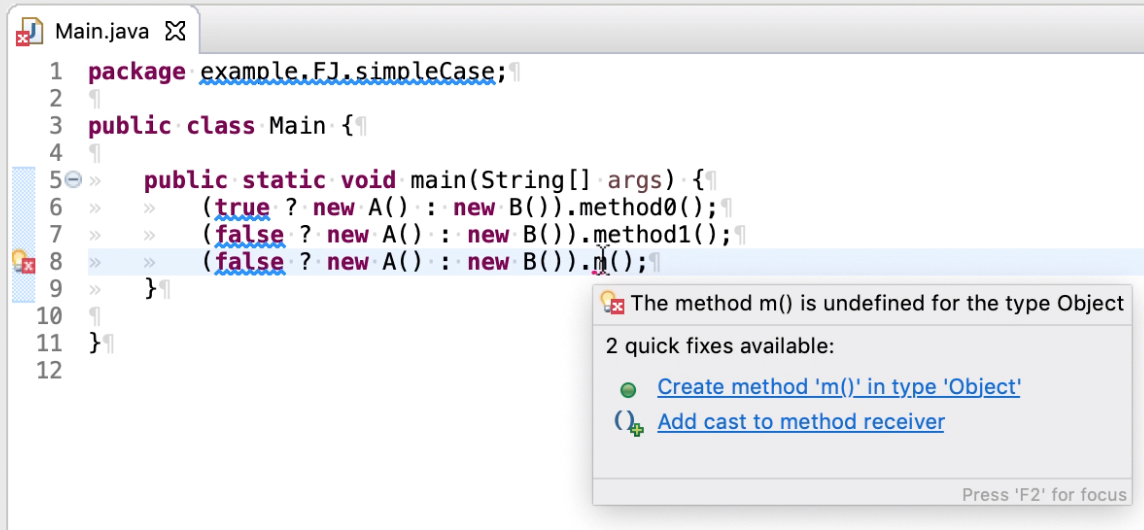
\includegraphics[width=1\linewidth]{images/example-normal-type.png}
\caption{Java correctly assigns the type \texttt{Object}.}
\label{fig:mainres}
\end{figure}
\end{frame}

\begin{frame}{Example 2}
		\framesubtitle{A set of interfaces without minimum common supertype}
	Consider $I_0,I_1,I_2,I_3$ interfaces.\newline
	Here the $join(I_2,I_3)$ it is not defined, since there is not  minimum common supertype.
	\begin{center}
		\begin{tikzpicture}[scale = 1.7]
		\node at (4,0)  (a3) {\LARGE$I_2$};
		\node at (4,1) (a1) {\LARGE$I_0$};
		\node at (5,1)  (a2) {\LARGE$I_1$};
		\node at (5,0)  (a4) {\LARGE$I_3$};
		\draw[thick, ->] (a4) -> (a1);
		\draw[thick, ->] (a4) -> (a2);
		\draw[thick, ->] (a3) -> (a1);
		\draw[thick, ->] (a3) -> (a2);
		\end{tikzpicture}
	\end{center}
	Figure: Example of a relationship between interfaces.
\end{frame}

\begin{frame}[fragile]{Example 2}
\boldmath
The body of the interfaces.	
\begin{flushleft}
\begin{lstlisting}[basicstyle=\scriptsize]
public interface I0 {
	public String method0();
}
public interface I1 {
	public String method1();
}
public interface I2 extends I0, I1 {
	public String method();
	public String method2();
}
public interface I3 extends I0, I1 {
	public String method();
	public String method3();
}
\end{lstlisting}
\end{flushleft}
\end{frame}


\begin{frame}[fragile]{Example 2}
\boldmath
The body of the classes.	
\begin{flushleft}
\begin{lstlisting}[basicstyle=\scriptsize]
public class A implements I2 {
	public String method0() {	return "A";	}
	public String method1() {	return "A";	}
	public String method() {	return "A";	}
	public String method2() {	return "A"; }
}

public class B implements I3 {
	public String method0() {	return "B"; }
	public String method1() {	return "B"; }
	public String method() {	return "B"; }
	public String method3() {	return "B"; }
}
\end{lstlisting}
\end{flushleft}
\end{frame}

\begin{frame}
\frametitle{Example 2}
Below, we show the Main.java class.
\begin{figure}
\centering
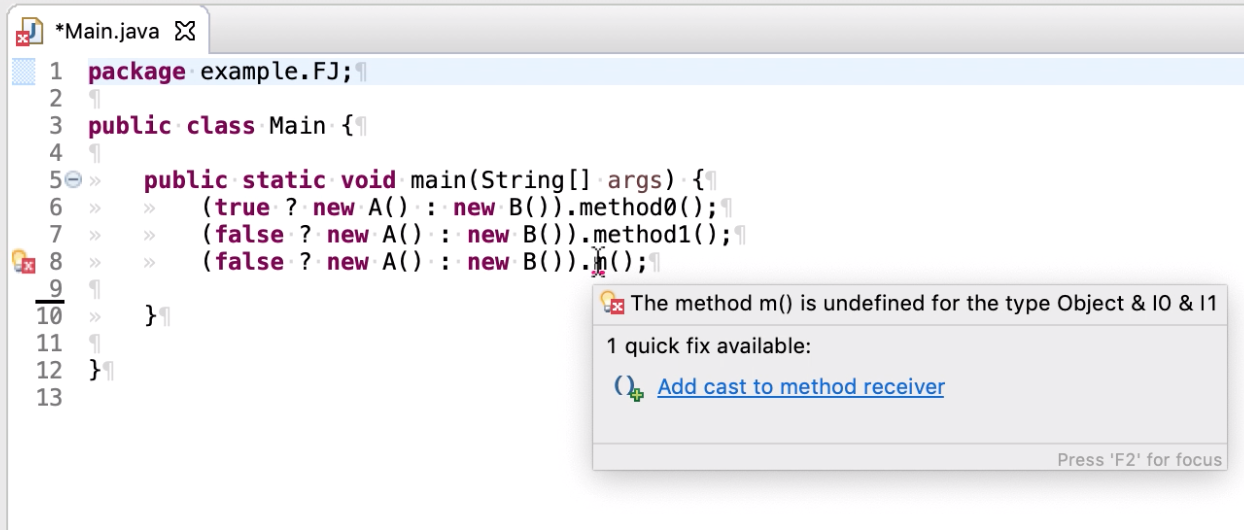
\includegraphics[width=1\linewidth]{images/example-intersection-type.png}
\caption{The type that Java creates to assign a type to the conditional expression is \texttt{(Object \& I0 \& I1)}.}
\label{fig:mainres}
\end{figure}
\end{frame}

\begin{frame}{Example 2}
	\begin{block}{What does it mean?}
    \textit{"The intersection type means having both one and the other specific of the interfaces involved, meaning that value is in the intersection of both, consequently with the conditional, if they don't have a minimum supertype common, I can make it with this.."}
\end{block}
\end{frame}


\begin{frame}{Example 3}
			\framesubtitle{Downcast intersection types with lambda expression}
			Consider $I_0,I_1$ interfaces.\newline
	\begin{center}
		\begin{tikzpicture}[scale = 1.7]
		\node at (4.5,1.5)  (a0) {\LARGE
			$(I_0\&I_1)$};
		\node at (3.5,0) (a1) {\LARGE
			$I_0$};
		\node at (5.5,0) (a2) {\LARGE
			$I_1$};

		\draw[thick, ->] (a1) -> (a0);
		\draw[thick, ->] (a2) -> (a0);
		\end{tikzpicture}
	\end{center}
Figure: We will see how Java create (and use) a new type.
\end{frame}

\begin{frame}[fragile]{Example 3}
\boldmath
The body of the functional interfaces.	
\begin{flushleft}
\begin{lstlisting}[basicstyle=\scriptsize]
@FunctionalInterface
public interface I0 {
	public int apply(int x);
	default void method0() {
		System.out.println("I0");
	}
}
@FunctionalInterface
public interface I1 {
	public int apply(int x);
	default void method1() {
		System.out.println("I1");
	}
}
\end{lstlisting}
\end{flushleft}
\end{frame}

\begin{frame}[fragile]{Example 3}
\boldmath
The body of the Main class.	
\begin{flushleft}
\begin{lstlisting}[basicstyle=\scriptsize]
public class Main {
	public static void main(String[] args) {
		var o = (I0 & I1) (x) -> (x + 1);
		System.out.println(o.apply(1));
		o.method0();
		o.method1();
		System.out.println(o.getClass().getName());
	}
}
\end{lstlisting}
\end{flushleft}
\end{frame}

\begin{frame}{Example 3}
Below, we show the Console after the compilation.
\begin{figure}
\centering
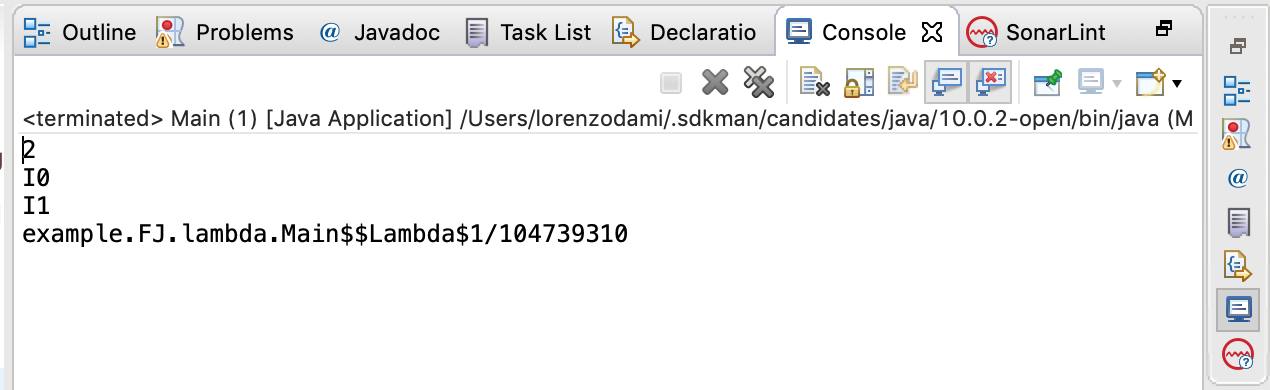
\includegraphics[width=1\linewidth]{images/downcast-java.png}
\caption{Still, i can invoke the method apply(), from the object made with intersection types, and i can invoke also both of the default method of the two previous classes.}
\label{fig:mainres}
\end{figure}
\end{frame}

\end{document}
